\documentclass[10pt,twocolumn]{IEEEtran}
\makeatletter
\def\subsubsection{\@startsection{subsubsection}
                                 {3}
                                 {\z@}
                                 {0ex plus 0.1ex minus 0.1ex}
                                 {0ex}
                             {\normalfont\normalsize\bfseries}}
\makeatother
\usepackage[T1]{fontenc}
\usepackage{subfigure}
\usepackage{ulem}
\usepackage{amsmath}
\allowdisplaybreaks
\usepackage{hhline}
\usepackage{yfonts,color}
\usepackage{soul,xcolor}
\usepackage{verbatim}
\usepackage{amsmath}
\allowdisplaybreaks
\usepackage{amssymb}
\usepackage{amsthm}
\usepackage{float}
\usepackage{bm}
\usepackage{url}
\usepackage{array}
\usepackage{cite}
\usepackage{graphicx}
\usepackage{tikz}
\usepackage{framed}
\usepackage{balance}
\usepackage{epsfig,epstopdf}
\usepackage{booktabs}
\usepackage{courier}
\usepackage{subfigure}
\usepackage{pseudocode}
\usepackage{enumerate}
\usepackage{algorithm}
\usepackage{algpseudocode}
\newtheorem{definition}{Definition}
\newtheorem{theorem}{Theorem}
\newtheorem{lemma}[theorem]{Lemma}
\newtheorem{proposition}[theorem]{Proposition}
\newtheorem{corollary}[theorem]{Corollary}
\newtheorem{assumption}{Assumption}
\newtheorem{remark}{Remark}
\renewcommand{\algorithmicrequire}{\textbf{Initialization:}}  
\renewcommand{\algorithmicensure}{\textbf{Output:}}  
\newcommand{\rom}[1]{\uppercase\expandafter{\romannumeral #1\relax}}
\usepackage{color}
\usepackage{soul,xcolor}
\newcommand{\sst}[1]{\st{#1}}
%\newcommand{\sst}[1]{}
\newcommand{\nm}[1]{{\color{blue}\bf{[NM: #1]}}}
%\newcommand{\nm}[1]{}
\newcommand{\bk}[1]{{\color{magenta}{[BK: #1]}}}
\newcommand{\nmmath}[1]{{\color{blue}\text{\bf{[NM: #1]}}}}
\newcommand{\gs}[1]{{\color{orange}\bf{[GS: #1]}}}
\newcommand{\remove}[1]{{\color{magenta}{\bf REMOVE: [#1]}}}
\DeclareMathOperator*{\argmax}{arg\,max}
\DeclareMathOperator*{\argmin}{arg\,min}
\usepackage{cancel}
\newcommand\mst[2][red]{\setbox0=\hbox{$#2$}\rlap{\raisebox{.45\ht0}{\textcolor{#1}{\rule{\wd0}{2pt}}}}#2} 
%\newcommand\mst[2][red]{} 
\newcommand{\add}[1]{{\color{red}{#1}}}
\newcommand{\ull}[1]{\textbf{\color{red}\ul{#1}}}
\normalem
\title{Spectrum Sensing in Cognitive Radio Networks
\\
via Approximate POMDP}
\author{Bharath Keshavamurthy, Nicol\`{o} Michelusi
\thanks{This research has been funded in part by NSF under grant CNS-1642982.}
\thanks{The authors are with the School of Electrical and Computer Engineering, Purdue University. email: \{bkeshava,michelus\}@purdue.edu.}
\vspace{-5mm}}
\begin{document} 
\setulcolor{red}
\setul{red}{2pt}
\maketitle
\setstcolor{red}
\begin{abstract}
Cognitive radio technologies will be critical to the wireless communication infrastructure due to their potential to alleviate the spectrum crunch, both in the commercial and the military spheres. In this paper, a novel spectrum sensing and access strategy based on Partially Observable Markov Decision Processes (POMDPs) is proposed, wherein a cognitive radio node learns the correlation model defining the occupancy behavior of the incumbents and devises an optimal strategy to perform spectrum sensing and access that exploits the learned correlation model.
To ameliorate the complexity of the POMDP optimization, the PERSEUS algorithm is employed, an approximate value iteration method.
\add{Numerical evaluations demonstrate that the proposed framework achieves the performance attained by a MAP-based state estimator with prior knowledge of the correlation model,
and outperforms a state-of-the art correlation-coefficient based clustering algorithm by an average of 80\%;
additionally,}
it surpasses a Neyman-Pearson Detector that assumes independence among channels, by an average of 24\%\add{, thus demonstrating the importance of leveraging the correlation structure definining the occupancy behavior of incumbents}.
\end{abstract}
\begin{IEEEkeywords}
Hidden Markov Model, Cognitive Radio, Spectrum Sensing, POMDP
\end{IEEEkeywords}
\section{Introduction}\label{I}
With the advent of fifth-generation wireless communication networks, the problem of spectrum scarcity has been exacerbated \cite{7158089}. For some time now, cognitive radio technologies have been in the spotlight as a potential solution to this problem in commercial and military applications. Cognitive radio networks facilitate efficient spectrum utilization by intelligently accessing \emph{white spaces} left unused by the sparse and infrequent transmissions of licensed users, while ensuring rigorous incumbent non-interference compliance \cite{4562537}. A crucial aspect underlying the design of cognitive radio networks is the channel access protocol in the MAC layer of the stack. In this regard, the current state-of-the-art involves channel access strategies dictated by multi-armed bandits \cite{7094730}, reinforcement learning agents \cite{6507570}, and other custom heuristics \cite{6956794, 4554696}. However, almost all these works, such as \cite{7094730, 6507570}, assume independence among channels in the discretized spectrum, which is imprudent because licensed users exhibit correlation across both frequency and time in their channel occupancy behavior: the primary users frequently occupy a set of adjacent channels (frequency correlation), repeating similar motifs in behavior over an extended period of time (temporal correlation) \cite{6188346, 4213046,McHenry:2006:CSO:1234388.1234389}. This pattern in occupancy behavior of the incumbents imputes very high levels of correlation among channels which need to be leveraged for more accurate predictions of spectrum holes. In this paper, we propose a parameter estimation algorithm to learn the aforementioned correlation model, and an approach to solve for the optimal channel sensing and access policy that exploits this learned correlation structure.

The works \cite{7094730, 7895211} develop spectrum sensing and access algorithms under the assumption that the occupancy behavior of incumbents is independent across both time and frequencies. In our work, we exploit both frequency and temporal correlations. In \cite{7336513}, a compressed spectrum sensing scheme is devised that exploits sparse temporal dynamics in the occupancy of licensed users, and in \cite{8571293}, an efficient spectrum sensing strategy is proposed for dense multi-cell cognitive networks, that also exploits the spatial structure of interference; however, both works assume independence across frequencies. Spectrum sensing and access strategies in a distributed multi-agent cognitive radio setting have been considered in \cite{6507570} and solved using SARSA with linear value function approximation. However, frequency correlation is precluded, and errors in state estimation are neglected in the decision process. Unlike \cite{6507570}, we consider a model with correlation across frequencies, and we account for uncertainty in the occupancy state via a POMDP formulation. Although the spectrum sensing algorithms detailed in \cite{6956794} consider the correlation in incumbent occupancy behavior across frequencies, the authors assume a perfect, noise-free observation model.
\add{Instead, we account for the impact of noisy observations in our design.} Other works model correlation across both time and frequencies, such as \cite{4554696}, \add{however} the algorithms operate based on a  data-driven strategy wherein pre-loaded databases are employed offline to estimate the correlation models. Instead, in our work,  we present a fully online framework that estimates the correlation models and simultaneously solves for the optimal channel sensing and access policy.

The rest of the paper is organized as follows: in Sec. \ref{II}, we define the signal model, followed by the formulations, approaches, and algorithms in Sec. \ref{III}; in Sec. \ref{IV}, we present numerical evaluations, followed by our conclusions in Sec. \ref{V}.
\section{System Model}\label{II}
\subsection{Signal Model}\label{A}
We consider a network consisting of $P$ licensed users termed the Primary Users (PUs) and one cognitive radio node termed the Secondary User (SU) equipped with a spectrum sensor. The objective of the SU is to opportunistically access portions of the spectrum left unused by the PUs in order to maximize its own throughput. To this end, the SU should learn 
how to intelligently access spectrum holes (white spaces) intending to maximize its throughput while maintaining strict non-interference compliance with incumbent transmissions.
The wideband signal received at the SU receiver at time $n$ is denoted as $y(n)$ and is given by 
\begin{equation}\label{1}
    y(n) = \sum_{p=1}^{P} \sum_{l=0}^{L_{p}-1} h_{p}(l)x_{p}(n-l) + v(n),
\end{equation}
where $y(n)$ is expressed as a convolution of the signal $x_{p}(n)$ of the $p$th PU with the channel impulse response $h_{p}(n)$, and $v(n)$ denotes additive white Gaussian noise (AWGN) with variances $\sigma_v^2$. Eq. (\ref{1}) can be written in the frequency domain by taking a $K$-point DFT which decomposes the observed wideband signal into $K$ discrete narrow-band components as 
\begin{equation}\label{2}
    Y_k(i) = \sum_{p=1}^{P} H_{p,k}(i)X_{p,k}(i) + V_k(i),
\end{equation}
where $i {\in} \{1,2,3,\dots,T\}$ represents the time index; $k {\in} \{1,2,3,\dots,K\}$ represents the index of the components in the frequency domain; $V_k(i) {\sim} \mathcal{CN}(0,\sigma_V^2)$ represents circularly symmetric additive complex Gaussian noise, i.i.d across frequency and across time, and independent of $H$ and $X$; $X_{p,k}(i)$ is the signal of the $p$th PU in the frequency domain, and $H_{p,k}(i)$ is its frequency domain channel. We further assume that the $P$ PUs employ an orthogonal access to the spectrum (e.g., OFDMA) so that $X_{p,k}(i)X_{q,k}(i)=0, \forall p\neq q$. Thus, letting $p_k$ be the index of the PU that contributes to the signal in the $k$th spectrum band, and letting  $H_{k}(i){=}H_{p_k,k}(i)$ and $X_{k}(i){=}X_{p_k,k}(i)$ (with $X_{k}(i){=}0$ if no PU is transmitting in the $k$th spectrum band at time $i$), we can rewrite \eqref{2} as 
\begin{equation}\label{3}
    Y_k(i) = H_{k}(i)X_{k}(i) + V_k(i).
\end{equation}
\sst{Thus, $H_k(i)$ represents the $k$th DFT coefficient of the impulse response $h_{p_k,k}(n)$ of the channel in between the PU operating on the $k$th spectrum band and the SU, at time $i$; }We model $H_{k}(i)$ as a zero-mean circularly symmetric complex Gaussian random variable with variance $\sigma_H^2$, $H_k {\sim} \mathcal{CN}(0,\sigma_H^2)$, i.i.d. across frequency bands, over time, and independent of the occupancy state of the channels.
\begin{figure}
    \centering
    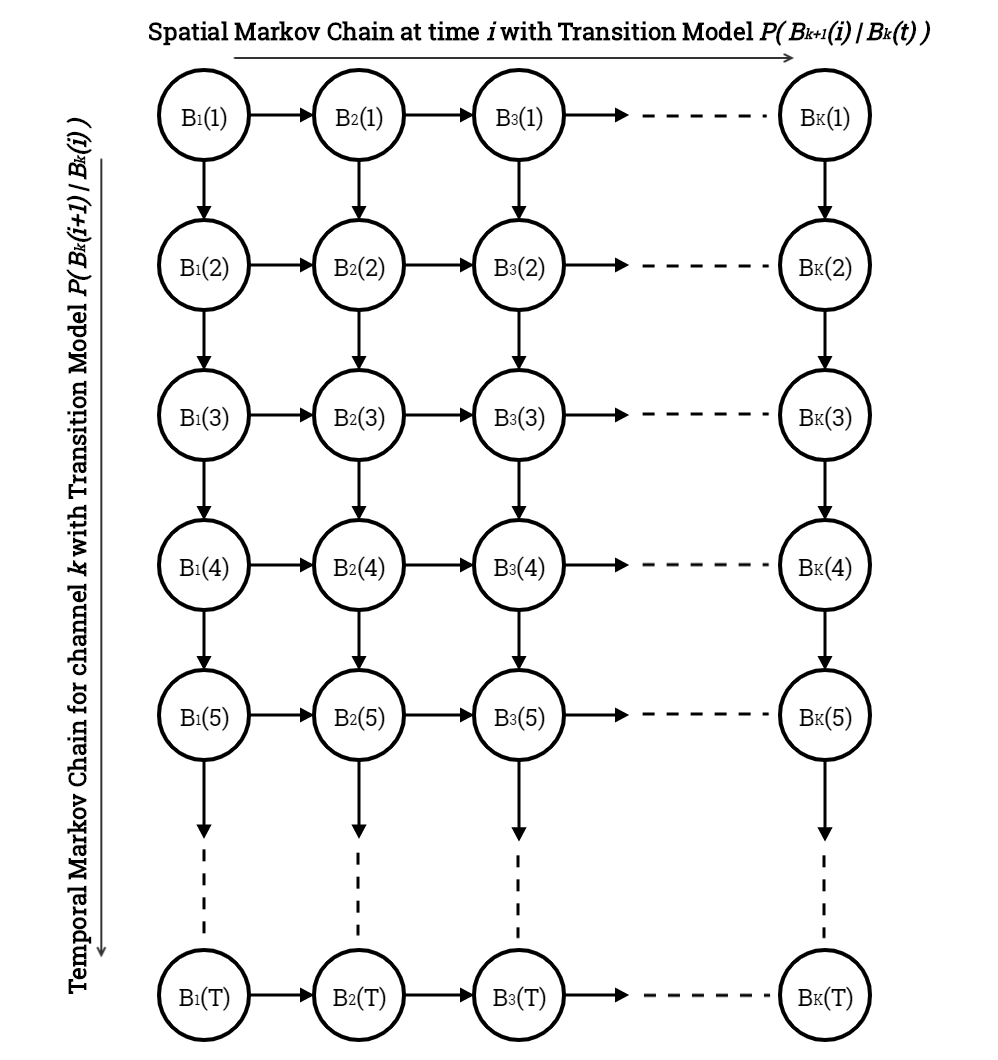
\includegraphics[width=.8\linewidth]{minerva_occupancy_markov_chain.png}
    \caption{The correlation model across time and frequencies underlying the occupancy behavior of incumbents in the network}
    \vspace{-5mm}
    \label{fig:1}
\end{figure}
\vspace{-3mm}
\subsection{PU Spectrum Occupancy Model}
We now introduce the model of PU occupancy over time and across the frequency domain. We model each $X_k(i)$ as 
\begin{equation}\label{4}
    X_k(i) = \sqrt{P_{tx}}B_k(i)S_k(i),
\end{equation}
where $P_{tx}$ is the transmission power of the PUs, $S_k(i)$ is the transmitted symbol modelled as a constant amplitude signal, $|S_k(i)|{=}1$, i.i.d. over time and across frequency bands;\footnote{In the case where $S_k(i)$ does not have constant amplitude, we may approximate $H_{k}(i)S_{k}(i)$ as complex Gaussian with zero mean and variance $\sigma_H^2\mathbb E[|S_{k}(i)|^2]$, without any modification to the subsequent analysis.} $B_k(i){\in}\{0,1\}$ is the binary spectrum occupancy variable, with $B_k(i){=}1$ if the $k$th spectrum band is occupied by a PU at time $i$, and $B_k(i){=}0$ otherwise. Therefore, the PU occupancy behavior in the entire wideband spectrum of interest at time $i$, discretized into narrow-band frequency components can be modeled as the vector 
\begin{equation}\label{5}
    \vec{B}(i) = [B_1(i), B_2(i), B_3(i), \cdots, B_K(i)]^T {\in} \{0, 1\}^K.
\end{equation}
PUs join and leave the spectrum at random times. To capture this temporal correlation in the spectrum occupancy dynamics of PUs, we model $\vec{B}(i)$ as a Markov process,
\begin{equation}\label{6}
    \begin{aligned}
        \mathbb{P}(\vec{B}(i+1)|\vec{B}(j), \forall j \leq i) = \mathbb{P}(\vec{B}(i+1)|\vec{B}(i)).
    \end{aligned}
\end{equation}
Additionally, when joining the spectrum pool, PUs occupy a number of adjacent spectrum bands, and may vary their spectrum needs depending on traffic demands, channel conditions, etc. To capture this behavior, we model $\vec{B}(i)$ as having Markovian correlation across spectrum bands,
\begin{align}\label{7}
&         \mathbb{P}(\vec{B}(i+1)|\vec{B}(i))\\&=
\nonumber
         \mathbb{P}(B_{1}(i+1)|B_{1}(i))
         \prod_{k=2}^{K} \mathbb{P}(B_{k}(i+1)|B_{k}(i), B_{k-1}(i+1)).
\end{align}
That is, the spectrum occupancy at time $i+1$ in frequency band $k$, $B_{k}(i+1)$, depends on the  occupancy state of the adjacent spectrum band at the same time, $B_{k-1}(i+1)$, and that of the same spectrum band $k$ in the previous time index $i$, $B_{k}(i)$ as shown in Fig. \ref{fig:1}.
\vspace{-3mm}
\subsection{Spectrum Sensing Model}
In order to detect the available spectrum holes, the SU performs spectrum sensing. However, owing to physical design limitations at the SU's spectrum sensor \cite{5990482},\sst{ not all channels in the discretized spectrum can be sensed at once:} the SU can sense only $\kappa$ out of $K$ spectrum bands at any given time,\nm{you never talk about this in the intro} with $1{\leq}\kappa{\leq}K$. Let $\mathcal K_{i}{\subseteq}\{1,2,\dots,K\}$ with $|\mathcal K_i|{\leq}\kappa$ be the set of indices of spectrum bands sensed by the SU at time $i$, which is part of our design.
Then, we define the observation vector
\begin{equation}\label{8}
    \vec{Y}(i) = [Y_k(i)]_{k {\in} \mathcal K_i},
\end{equation}
where $Y_k(i)$ is given by \eqref{3}.
The true states $\vec{B}(i)$ encapsulate the actual occupancy behavior of the PU and the measurements at the SU are noisy observations of these true states which are modeled to be the observed states of a Hidden Markov Model (HMM). 
Conditional on $\vec{B}(i)$ and $\mathcal K_i$, the probability density function of $\vec{Y}(i)$ is expressed as
\begin{equation}\label{9}
    f(\vec{Y}(i)|\vec{B}(i), \mathcal K_i) = \prod_{k \in \mathcal K_i} f(Y_k(i)|B_k(i)),
\end{equation}
owing to the independence of channels, noise, and transmitted symbols across frequency bands. Moreover, from \eqref{3},
\begin{equation}\label{10}
 Y_k(i)|B_k(i) \sim \mathcal{CN}(0, \sigma_H^2P_{tx}B_k(i) + \sigma_V^2).
\end{equation}
\subsection{POMDP Agent Model}
In this section, we model the spectrum access scheme of the SU as a POMDP, whose goal is to devise an optimal sensing and access policy in order to maximize its throughput while maintaining strict non-interference compliance with incumbent transmissions. In fact, the agent's limited sensing capabilities coupled with its noisy observations result in an increased level of uncertainty at the agent's end about the occupancy state of the spectrum under consideration and the exact effect of executing an action on the radio environment. The transition model of the underlying MDP as described by \eqref{7}, is denoted by $\mathbf{A}$ and is learned by the agent by interacting with the radio environment (see Sec. \ref{III}). The emission model is denoted by $\mathbf{M}$ and is given by \eqref{9}, with $f(Y_k(i)|B_k(i))$ given by \eqref{10}. 

We model the POMDP as a tuple $(\mathcal B,\mathcal{A},\mathcal{Y},\mathbf{A},\mathbf{M})$ where $\mathcal{B}\equiv\{0,1\}^K$ represents the state space of the underlying MDP with states $\vec{B}$ given by all possible realizations of the spectrum occupancy vector as described by \eqref{5}, $\mathcal{A}$ represents the action space of the agent, given by all possible combinations in which the $\kappa$ spectrum bands are chosen to be sensed out of $K$ at any given time; and $\mathcal{Y}$ represents the observation space of the agent based on the signal model outlined in the previous \sst{sub}section.\nm{never use subsection in the main text} 
The state of the POMDP at time $i$ is given by the \emph{prior belief} $\beta_i$, which represents the probability distribution of the underlying MDP state $\vec{B}(i)$, given the information collected by the agent up to time $i$, but before collecting the new information in slot $i$. At the beginning of each time index $i$, given $\beta_i$, the agent selects $\kappa$ spectrum bands out of $K$ according to a policy $\pi(\beta_i)$, thus defining the sensing set $\mathcal K_i$, performs spectrum sensing  on these spectrum bands, observes $\vec{Y}(i){\in} \mathcal{Y}$, and updates its \emph{posterior belief} $\hat{\beta}_i$ of the current spectrum occupancy $\vec{B}(i)$ as 
\begin{align}\label{11}
\hat\beta_i(\vec{B}') &= \mathbb{P}(\vec{B}(i) = \vec{B}'|\vec{Y}(i), \mathcal K_i, \beta_i)\\&=
\nonumber
\frac{\mathbb{P}(\vec{Y}(i)|\vec{B}', \mathcal{K}_i) \beta_i(\vec{B}')}{
\sum_{\vec{B}'' {\in} \{0,1\}^K} \mathbb{P}(\vec{Y}(i)|\vec{B}'', \mathcal{K}_i) \beta_i(\vec{B}'')}.
\end{align}
We denote the function that maps the prior belief $\beta_i$ to the posterior belief $\hat\beta_i$ through the spectrum sensing action $\mathcal K_i$ and the observation signal $\vec{Y}(i)$ as $\hat\beta_i=\hat{\mathbb B}(\beta_i, \mathcal K_i, \vec{Y}(i))$.

Given the posterior belief $\hat{\beta}_i$, we estimate the occupancy state of the discretized spectrum under consideration as
\begin{equation}
    \vec{B}(i)^{*} = \argmax_{\vec{B} {\in} \mathcal{B}} \hat{\beta}_{i}(\vec{B}).
\end{equation}
Let $B_{k}(i)^{*} = \phi_{k}(\hat{\beta}_{i}) {\in} \{0, 1\}$ be the \add{estimated} state of channel $k$ at time $i$. If the channel is deemed to be idle as a result of this MAP estimation procedure, i.e., $\phi_{k}(\hat{\beta}_{i}) = 0$, the SU accesses the channel for delivering its network flows. Else, it leaves it untouched. Given the PU occupancy state $\vec{B}(i)$ and posterior belief $\hat\beta_i$, the reward metric of the POMDP is given by the number of \emph{truly idle} bands detected by the SU accounting for the throughput maximization aspect of the agent's objective and a penalty for \emph{missed detections} accounting for the incumbent non-interference constraint, i.e.,
\begin{equation}
\nonumber
    R(\vec{B}(i), \hat{\beta}_i){=}\sum_{k=1}^{K} (1{-}B_k(i))(1{-}\phi_k(\hat{\beta}_{i})){-}\lambda B_k(i)(1 - \phi_k(\hat{\beta}_i)),
\end{equation}
where $\lambda{>}0$ represents \add{a penalty factor}\sst{
 the cost term penalizing the agent for missed detections, i.e. interference with the incumbent}. After performing data transmission, the SU computes the prior belief for the next slot based on the dynamics of the Markov chain as
\begin{equation}\label{13}
    \beta_{i+1}(\vec{B}') = \mathbb{P}(\vec{B}(i+1) = \vec{B}'|\hat{\beta}_{i}).
\end{equation}
We denote the function that maps the posterior belief $\hat\beta_i$ to the prior belief $\hat\beta_{i+1}$ as $\beta_{i+1}={\mathbb B}(\hat\beta_i)$.
The goal of the problem at hand is to determine an optimal spectrum sensing policy to maximize the infinite-horizon discounted reward,
\begin{equation}\label{14}
    \pi^{*}{=}\argmax_{\pi} V^{\pi}(\beta) \triangleq \mathbb{E}_{\pi} \Big[\sum_{i=1}^{\infty} \gamma^{i} R(\vec{B}(i), \hat{\beta}_i)|\beta_0 {=}\beta\Big],
\end{equation}
where $0{<}\gamma{<}1$ is the discount factor, $\beta_0$ is the initial belief, and $\hat\beta_i$ is the posterior belief induced by policy $\add{\mathcal K_i{=}}\pi\add{(\beta_i)}$ \add{and the observation $\vec{Y}(i)$ via $\hat\beta_i{=}\hat{\mathbb B}(\beta_i, \mathcal K_i, \vec{Y}(i))$}\sst{, which maps the beliefs $\beta_i$ to actions $\mathcal{K}_i$ at time $i$}, and we have defined the value function $V^{\pi}(\beta)$ under policy $\pi$ starting from belief $\beta$.
The optimal policy $\pi^*$ and the corresponding optimal reward $V^*(\beta)$ are the solutions of Bellman's optimality equation $V^*{=}H[V^*]$, where the operator $V_{n+1}{=}H[V_n]$ is defined as
\begin{align}\label{16}
\nonumber
        V_{n+1}(\beta) = &\max_{\mathcal{K} {\in} \mathcal{A}} \sum_{\vec{B} {\in} \mathcal{B}} \beta(\vec{B}) \mathbb{E}_{\vec{Y}|\vec{B}, \mathcal{K}} \Big[R(\vec{B}, \hat{\mathbb{B}}(\beta, \mathcal{K}, \vec{Y}))\\ &+\gamma V_n(\mathbb{B}(\hat{\mathbb{B}}(\beta, \mathcal{K}, \vec{Y})))\Big],\ \forall \beta.
\end{align}

This problem can be solved using the value iteration algorithm, i.e., by solving \eqref{16} iteratively until convergence to a fixed point. However, given the high dimensionality of the spectrum sensing and access problem, i.e. the number of states of the underlying MDP scales exponentially with the number of bands in the spectrum, solving equation \eqref{16} using Exact Value Iteration and Policy Iteration algorithms is computationally infeasible. Additionally, solving for the optimal policy from equation \eqref{16} requires prior knowledge about the underlying MDP's transition model. Therefore, in this paper we present a framework to estimate the transition model of the underlying MDP online, while simultaneously utilizing this learned model to solve for the optimal policy by employing randomized point-based value iteration techniques, namely, the PERSEUS algorithm \cite{DBLP:journals/corr/abs-1109-2145}.
\vspace{-3mm}
\section{Approaches and Algorithms}\label{III}
\subsection{Occupancy Behavior Transition Model Estimation}
In real-world implementations of cognitive radio systems, the transition model of the occupancy behavior of the PUs is unknown to the SUs in the network and needs to be learned over time. The learned model then needs to be fed back to the POMDP agent which is solving for the optimal spectrum sensing and access policy simultaneously. Inherently, the approach constitutes in solving the Maximum Likelihood Estimation (MLE) problem
\begin{equation}\label{17}
    \mathbf{A}^{*} = \argmax_{\mathbf{A}} \mathbb{P}([\vec{Y}(i)]_{i=1}^{\tau}|\mathbf{A}),
\end{equation}
where $\mathbf{A}$ is \add{the transition model} defined as $\mathbb{P}(\vec{B}(i+1)|\vec{B}(i))$ and $\tau$ refers to the learning period of the parameter estimator: this can be equal to the entire duration of the POMDP agent's interaction with the radio environment implying simultaneous model learning or can be a predefined parameter learning period before triggering the POMDP agent. In order to facilitate better readability, for the description of this parameter estimator, we denote $[\vec{Y}(i)]_{i=1}^{\tau}$ as $\mathbf{Y}$ and $[\vec{B}(i)]_{i=1}^{\tau}$ as $\mathbf{B}$. Re-framing \eqref{17} as an optimization of the log-likelihood, we get,
\begin{equation}\label{18}
    \mathbf{A} = \argmax_{\mathbf{A}} \log\Big(\sum_{\mathbf{B}} \mathbb{P}(\mathbf{B}, \mathbf{Y}| \mathbf{A})\Big).
\end{equation}
This problem can be solved using the Expectation-Maximization algorithm, where the E-step constitutes
\begin{equation}
    Q(\mathbf{A}|\hat{\mathbf{A}}^{(t)}) = \mathbb{E}_{\mathbf{B}|\mathbf{Y}, \hat{\mathbf{A}}^{(t)}} \Big[ \log \Big(\sum_{\mathbf{B}} \mathbb{P}(\mathbf{B}, \mathbf{Y}|\hat{\mathbf{A}}^{(t)}) \Big) \Big],
\end{equation}
and the M-step constitutes
\begin{equation}
    \hat{\mathbf{A}}^{(t+1)} = \argmax_{\mathbf{A}} Q(\mathbf{A}|\hat{\mathbf{A}}^{(t)}).
\end{equation}
In order to solve for $a_{LR} {\in} \mathbf{A}$\nm{what do you mean by $a_{LR} {\in} \mathbf{A}$?? Is $\mathbf A$ a set? (it is not).. what does $a_{LR}$ represent? Didn't we assume that $\mathbf A$ is just parameterized by two parameters $p$ and $q$ modeling the frequency and time correlation?} where, $L, R {\in} \{0, 1\}^{K}$ and bring the solution into a simplified iterative form, we use the forward and backward probability members\nm{members? what is it?} defined as
\begin{align}
        F(i,R) &= \mathbb{P}([\vec{Y}(t)]_{t=1}^{i},\vec{B}(i)=R)\\
        &= 
        \sum_{L}\mathbb{P}(\vec{B}(i)=R,\vec{Y}(i)|\vec{B}(i-1)=L)F(i-1,L),
        \nonumber
        \\
        D(i,L) &= \mathbb{P}([\vec{Y}(t)]_{t=i}^{\tau}|\vec{B}(i-1)=L)\\
        &= \sum_{R}\mathbb{P}(\vec{B}(i)=R,\vec{Y}(i)|\vec{B}(i-1)=L)D(i+1,R).
                \nonumber
\end{align}
\nm{How do you compute these probabilities if these probabilities are not even available since you are estimating then? Where is this coming from?}
Using these definitions, the iterative procedure turns out to be,
\begin{equation}
\nonumber
    a_{LR}^{(t+1)}{=}\frac{\sum_{i=1}^{\tau}F(i-1,L)\mathbf{M}_R(\vec{Y}(i))a_{LR}^{(t)}D(i+1,R)}{\sum_R\sum_{i=1}^{\tau}F(i-1,L)\mathbf{M}_R(\vec{Y}(i))a_{LR}^{(t)}D(i+1,R)},
\end{equation}
\nm{again, $F$ and $D$ depends on probabilities that you are trying to estimate.. this does not make sense..}
until the convergence condition $|a_{LR}^{(t+1)} - a_{LR}^{(t)}| \leq \epsilon$ is satisfied, where $\epsilon > 0$, a very small quantity.

\nm{I thought that in your model the PU transitions are defined by a time correlation parameter $p$ and a frequecny correlation parameter $q$, but here you are not using that model.. which one is that you are using in your numerical results?}
\subsection{The PERSEUS Algorithm}
As discussed in Sec. \ref{II} of this article, solving the Bellman equation \eqref{16} for POMDPs with large state and action spaces using exact value iteration and policy iteration techniques is computationally infeasible \cite{DBLP:journals/corr/abs-1109-2145}. Hence, we resort to approximate value iteration techniques to ensure that the system scales well to a large number of bands in the spectrum of interest. For infinite-horizon POMDPs, $V^*$ in \eqref{16} can be approximated by a Piece-Wise Linear and Convex function (PWLC) \cite{DBLP:journals/corr/abs-1109-2145}. The core idea behind the PERSEUS algorithm is that the value function at time index $i$ can be parameterized by a set of hyperplanes $\{\vec{\alpha}_i^{u}\}$, $u = \{0,1,2,\dots,|V_i|\}$,\nm{you are using $V_i$ for value function, dont use it for number of hyperplanes as well} each of which represents a region of the belief space for which it is the maximizing element. The backup step is defined as the process of determining the optimal hyperplane out of the set of available hyperplanes in time index $i$ as
\begin{equation}\label{39}
    \vec{\alpha}_{i}(\beta) = \argmax_{\vec{\alpha}_{i}^u, u {\in} \{0, 1, 2, \dots, |V_i(\beta)|\}} \beta \cdot \vec{\alpha}_{i}^u,
\end{equation}
which implies that,
\begin{equation}\label{40}
        V_i(\beta) =\!\!\!\!\!\max_{\vec{\alpha}_{i}^u, u {\in} \{0, 1, 2, \dots, |V_i(\beta)|\}} \beta \cdot \vec{\alpha}_{i}^u,
\ \ \pi_i(\beta) = a(\vec{\alpha}_i^{u*}),
\end{equation}
\nm{what is $|V_i(\beta)|$? Please be carefuly with your notation! $V_i(\beta)$ is a value function, NOT a number of elements within a set!}
where $a(\vec{\alpha}_i^{u})$ is the action corresponding to hyperplane $\vec{\alpha}_i^{u}$. The set of available hyperplanes is a collection of policy trees, where $\vec{\alpha}_{i} \equiv [V_{i}(\vec{B}): \vec{B} \in \mathcal{B}]$.\nm{this is unclear.. introduce the updates for the hyperplanes} PERSEUS is a randomized point-based value iteration algorithm whose goal is to improve the value of all belief point\nm{are you sure about the "all" belief points? It improves only the value on belief points in a discrete set!} by updating the value and gradient\nm{the gradient? why?} of only a subset of these belief points, chosen at random. The procedure constitutes an initial phase wherein the POMDP agent randomly interacts with the radio environment to collect a set of so-called \emph{reachable beliefs} which are to be improved over numerous iterative backup stages. In each backup stage, the agent samples a belief $\beta$ uniformly at random from the set of unimproved points and performs a backup on this sampled belief point according to \eqref{39}, to determine the optimal hyperplane, i.e., policy tree. Considering an arbitrary time index $i$, if $V_{i+1}(\beta) = \beta \cdot \vec{\alpha} \geq V_{i}(\beta)$, then the belief point $\beta$ is said to be improved along with any other belief points $\beta'$ in the unimproved set for which $V_{i+1}(\beta') = \beta' \cdot \vec{\alpha} \geq V_{i}(\beta')$. If $V_{i+1}(\beta) = \beta \cdot \vec{\alpha} < V_{i}(\beta)$, then a copy of the maximizing hyperplane for $V_i(\beta)$ is used for $V_{i+1}(\beta)$ and the belief point $\beta$ is then removed from the set of unimproved points. The backup stage continues until the set of unimproved points is empty and the agent performs a series of backup stages until there the number of policy changes between consecutive iterations is below a specified threshold $\eta$.

The belief update procedure outlined in \eqref{11} is an essential aspect of the PERSEUS algorithm which can turn into a performance bottleneck for large state spaces due to the inherent iteration over all possible states. In order to circumvent this problem, we fragment the spectrum into much smaller, independent sets of correlated channels and then run the PERSEUS algorithm on these fragments by leveraging multi-processing and multi-threading tools available at our disposal in software frameworks. Furthermore, we avoid iterating over all possible states and allow only those state transitions we deem to be the most probable - for example, we allow only those state transitions that involve a Hamming distance of up to 3 between the previous state vector and the current state vector in an 18 channel radio environment.
\section{Numerical Evaluation}\label{IV}
\begin{figure}
    \centering
    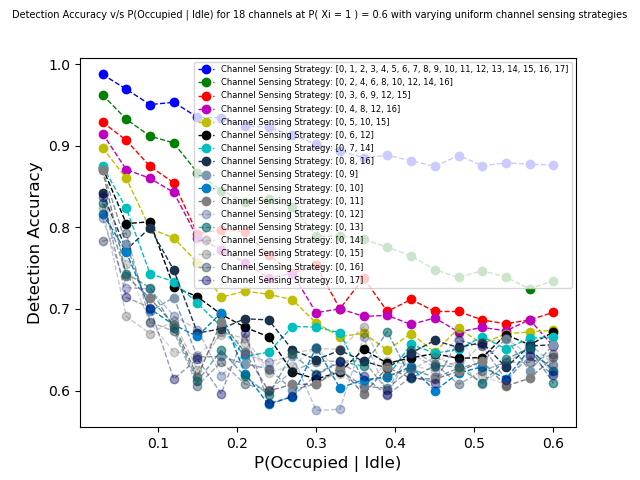
\includegraphics[width=.8\linewidth]{Uniform_Channel_Sensing.png}
    \caption{The detection accuracies of the constrained Viterbi algorithm for different sensing strategies over varying values of $\mathbb{P}(\text{Occupied}|\text{Idle})$}
    \label{fig:2}
\end{figure}
\nm{you have a super long paragraph here.. please break it down into smaller ones}
The given framework is simulated in Python for a system with 18 channels and a channel model constituting an SNR of 19dB when an incumbent occupies a specific channel. The same\nm{what do you mean by the same? The same as what?} Markovian transition model, emission model, and steady-state model is employed across both the chain across time and the chain across frequencies. The first line trace (in blue) depicted in Fig. \ref{fig:2} illustrates the detection accuracies of the Viterbi algorithm\nm{you never mentioned the Viterbi algorithm before and now it is coming out of the blue.. you need to introduce it first and motivate why you consider this algorithm.. Are you using it as part of Perseus? Or is it just for comparison?} wherein the SU makes observations of all the channels in the radio environment and estimates the occupancy states of these channels over varying values of $\mathbb{P}(\text{Occupied}|\text{Idle})$, i.e., as the channels transition toward independence. We note that the detection accuracy of this MAP-based state estimator degrades as the channels transition toward independence, which is as surmised, because the Viterbi algorithm's structure begins to crumble if the Markovian correlation ceases to exist among cells in the grid, where a cell corresponds to the state of a certain channel at a given time index. This plot is an important illustration to prove that leveraging correlation in incumbent occupancy behavior across both time and frequencies gives us a boost in detection accuracy, and thereby, a boost in secondary network throughput while complying with the required non-interference constraints.
\begin{figure}
    \centering
    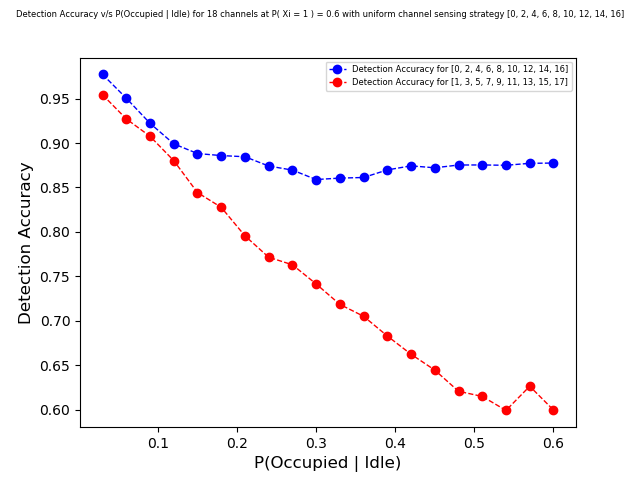
\includegraphics[width=.8\linewidth]{Uniform_Channel_Sensing_1.png}
    \caption{The detection accuracies of the constrained Viterbi algorithm for sensed and un-sensed channels under a given channel sensing strategy}
    \label{fig:3}
\end{figure}
Fig. \ref{fig:2} also illustrates the detection accuracies of the Viterbi algorithm (refer to all the other line traces) wherein the SU makes observations of only the channels in the given channel sensing strategy and estimates the occupancy states of all the channels in the discretized spectrum of interest over varying values of $\mathbb{P}(\text{Occupied}|\text{Idle})$. In Fig. \ref{fig:3}, the plot differentiates the trend in detection accuracies for the sensed and the un-sensed channels in relation to a constrained Viterbi algorithm in which the SU only senses channels whose indices correspond to the multiples of 2 and uses these channels to estimate the occupancy behavior of the incumbents across all 18 channels over varying values of $p = \mathbb{P}(\text{Occupied}|\text{Idle})$. In both these plots i.e., Fig. \ref{fig:2} and \ref{fig:3}, we observe that, as anticipated, the detection accuracy of this MAP-based state estimator deteriorates as the amount of information available for estimation decreases. These plots illustrate that the imposition of sensing limitations on the SU's spectrum sensor in view of quick turnaround times and improved energy efficiency, will put a dent in the detection accuracy of the cognitive radio node, and this needs to be addressed by leveraging the correlation in incumbent occupancy behavior across both time and frequencies.
\begin{figure}
    \centering
    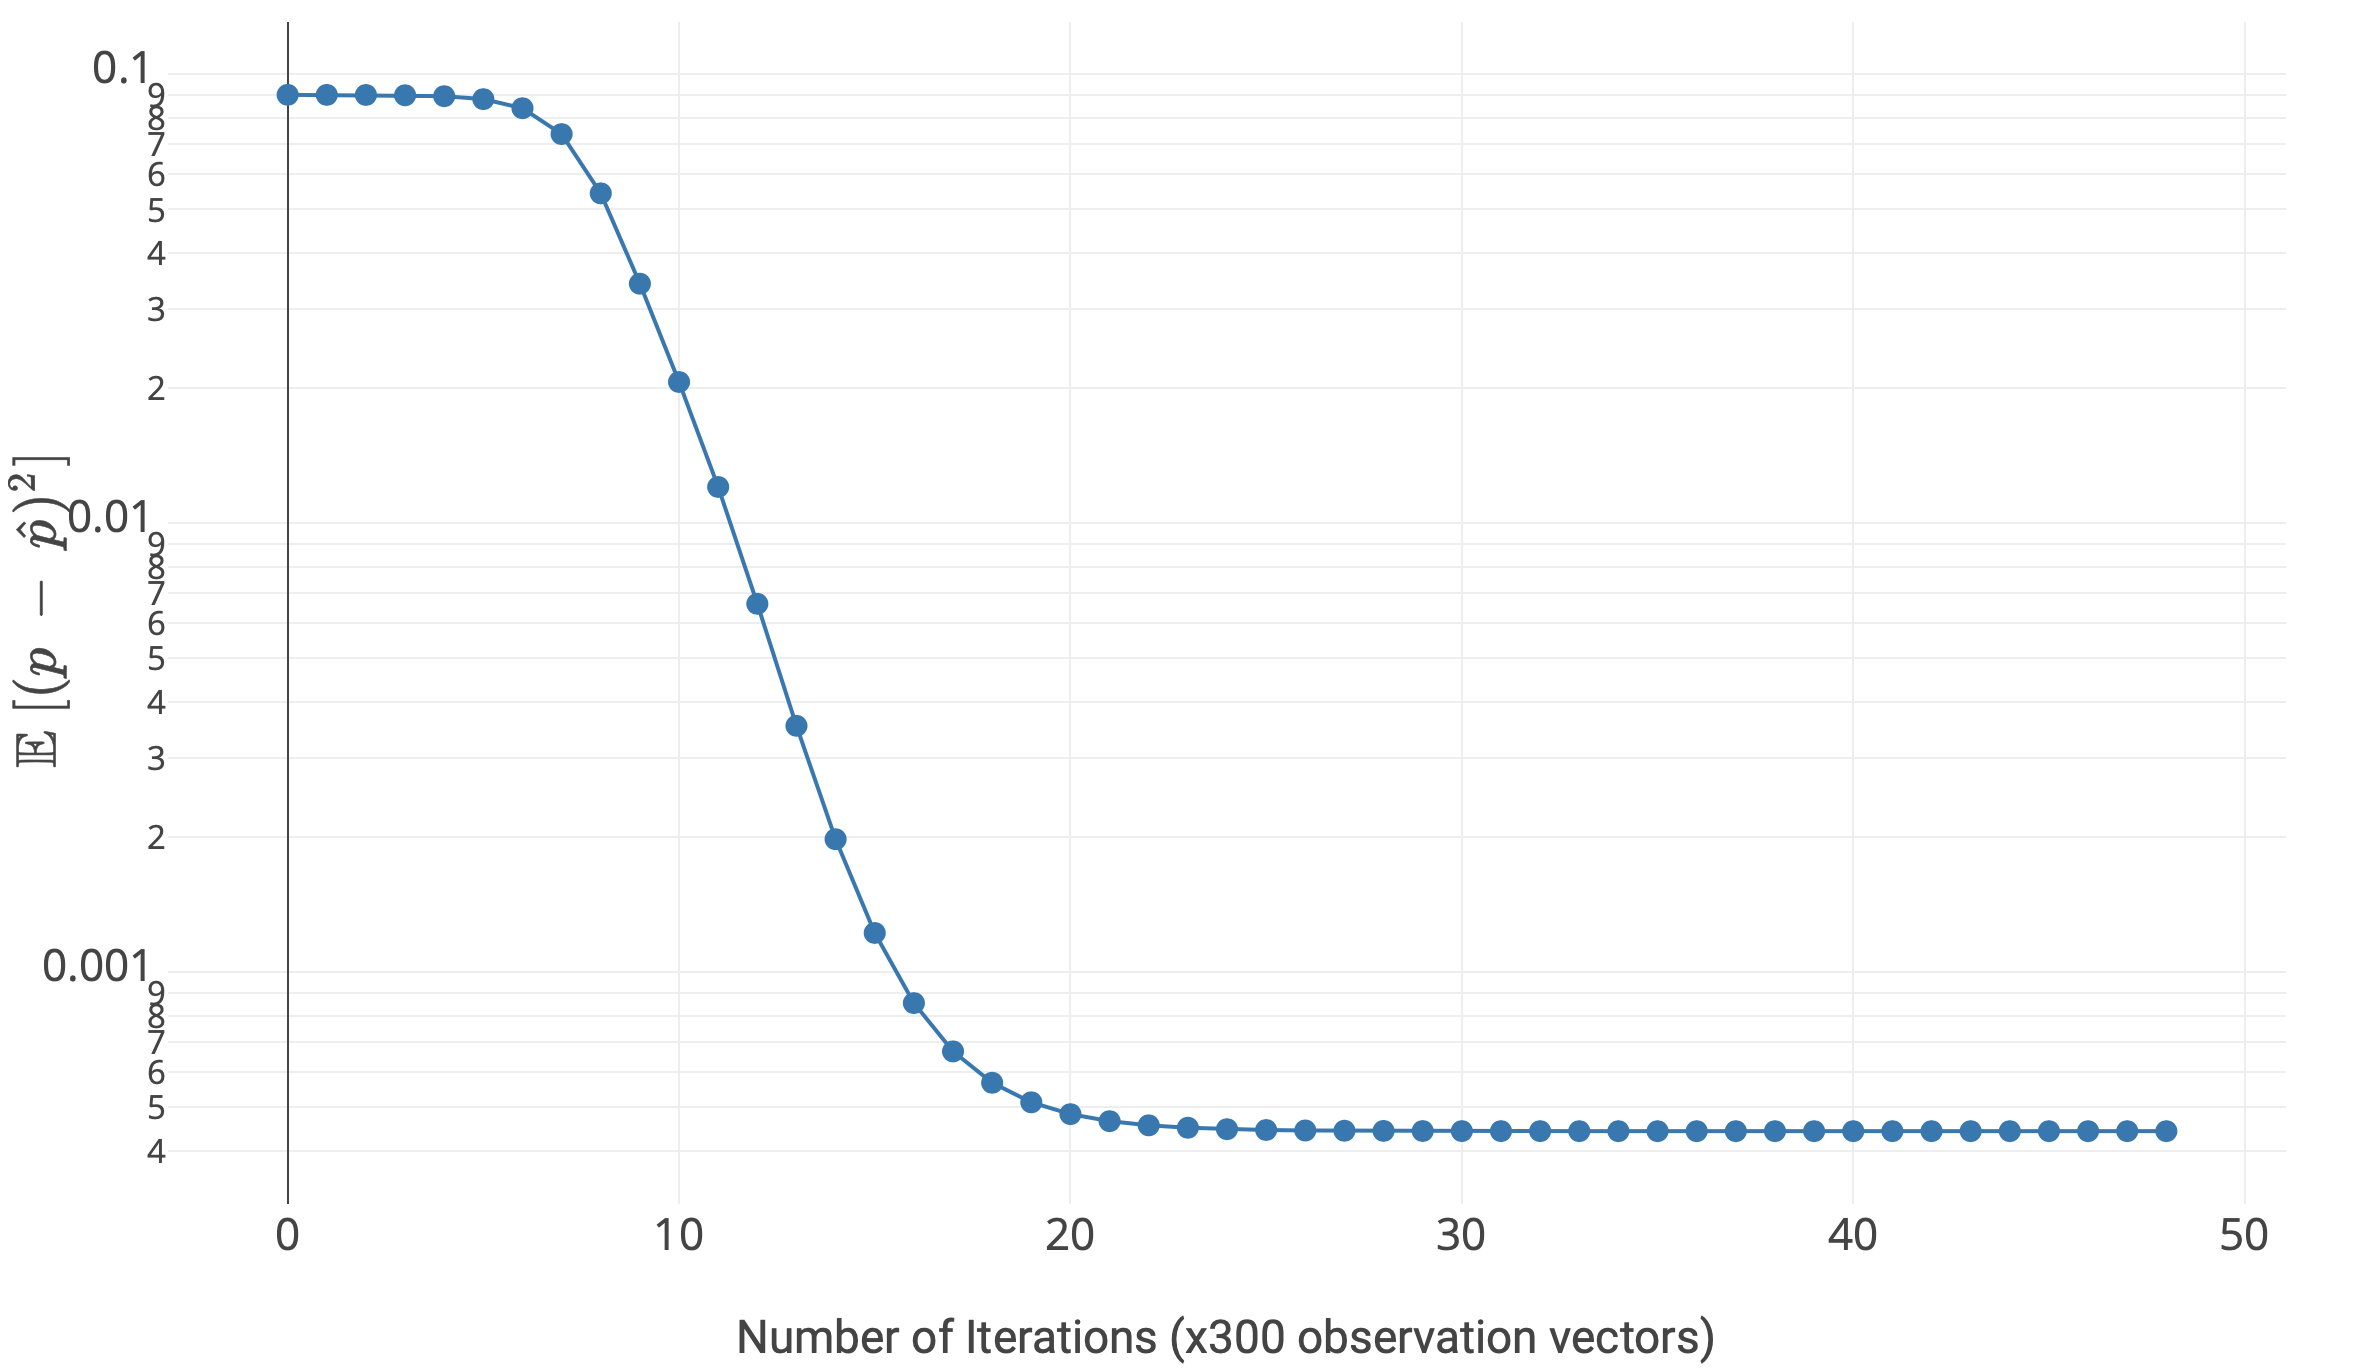
\includegraphics[width=.8\linewidth]{ParameterEstimatorConvergence.png}
    \caption{The mean square error convergence plot of the parameter estimation algorithm\nm{what are the parameteres that you are estimating here?}}
    \label{fig:4}
\end{figure}

The plot depicted in Fig. \ref{fig:4} shows the Mean Square Error convergence of the Parameter Estimation algorithm while determining the transition model of the MDP underlying the problem under consideration. Starting with an initial estimate of 0.0, the EM algorithm detailed in Sec. \ref{III} converges to the true transition model  with an error of $\epsilon \leq 10^{-8}$ over numerous iterations, each iteration corresponding to an averaging operation constituting 300 observation vectors. Here, we observe the mean square error given by $\mathbb{E}[(p - \hat{p})^{2}]$ iteratively reduces as it goes through the E-step which finds the distribution for the parameters in the current time-step, given the previous estimate and the M-step which determines the maximum likelihood estimate of the parameters, given the distribution obtained in the E-step. It has been theoretically shown to converge, i.e., each iteration either improves the true likelihood or leaves it unchanged \cite{Neal1998}. Since the EM algorithm is susceptible to premature convergence to local optima and saddle points, we mitigate this by averaging the procedure over several cycles.
\begin{figure}
    \centering
    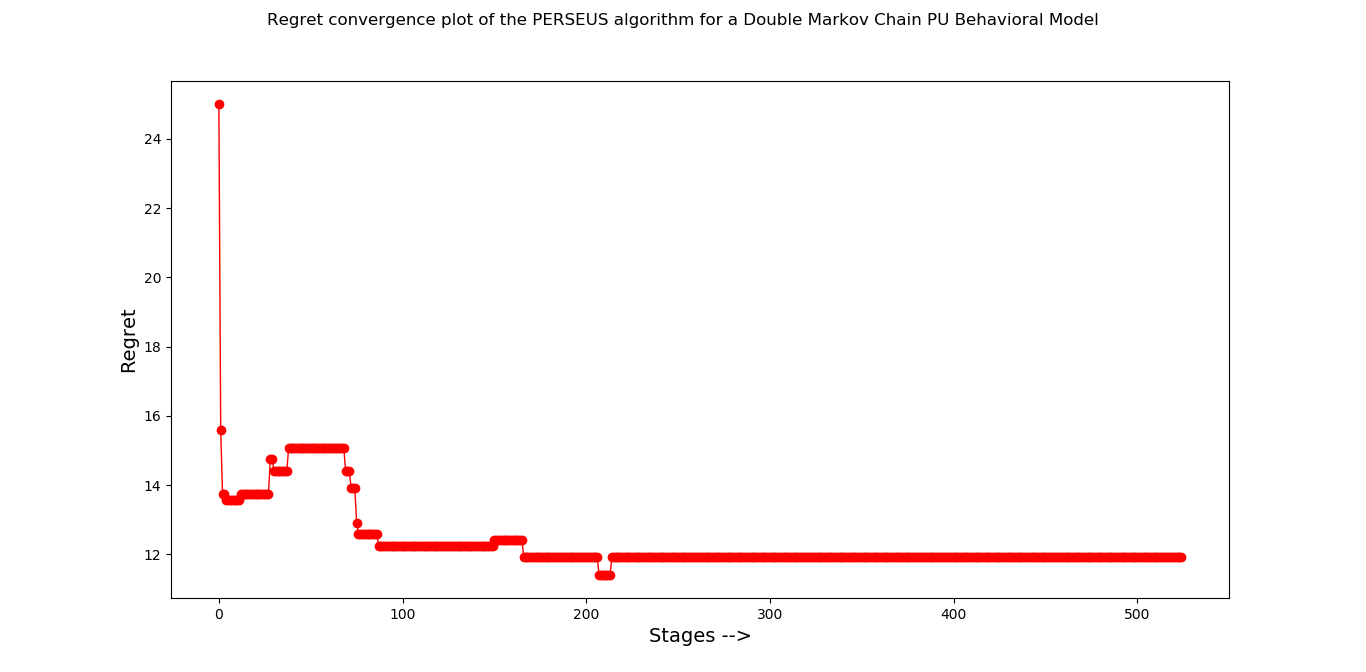
\includegraphics[width=.8\linewidth]{Regret_Convergence_Plot_04112019.png}
    \caption{The regret convergence plot of the PERSEUS algorithm over several backup and wrapper stages}
    \label{fig:5}
\end{figure}
\begin{figure}
    \centering
    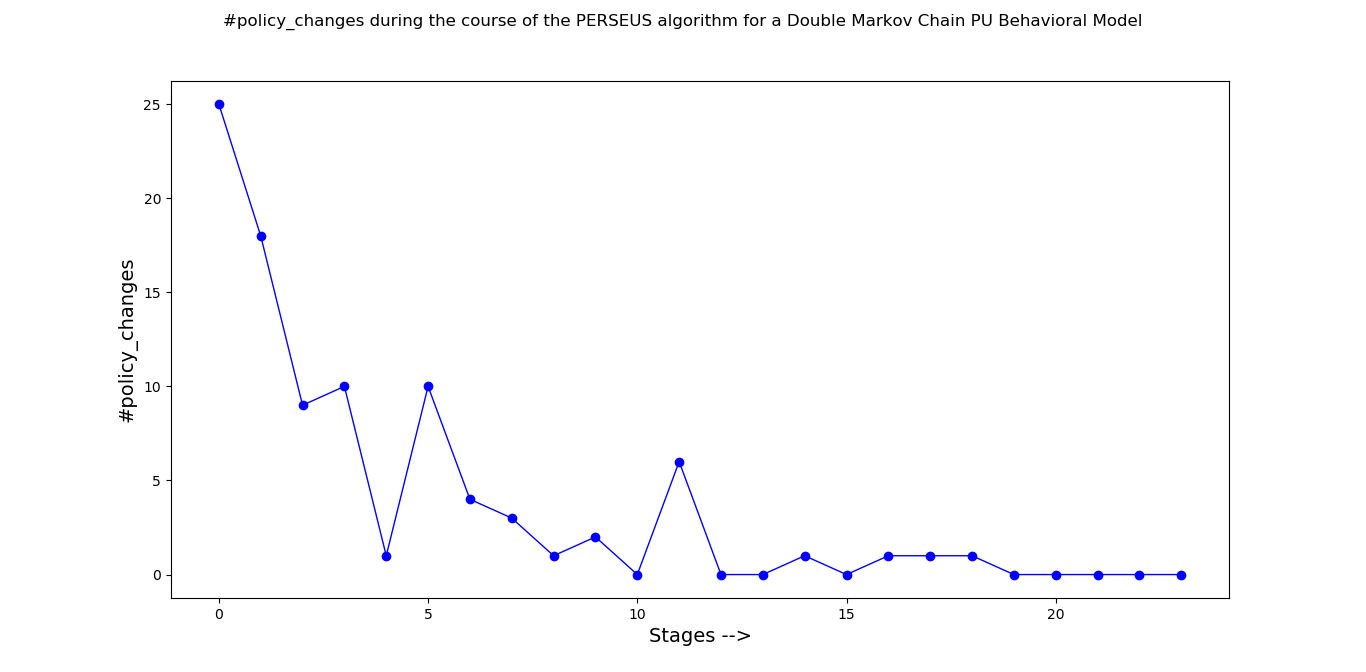
\includegraphics[width=.8\linewidth]{Policy_Changes_Plot_04112019.png}
    \caption{The number of policy changes involved in the PERSEUS algorithm as it transitions toward convergence over numerous backup and wrapper\nm{I dont think you have defined a wrapper stage..what is it?} stages}
    \label{fig:6}
\end{figure}

Fig. \ref{fig:5} illustrates the Regret Convergence plot of the PERSEUS algorithm over several backup and wrapper stages wherein the regret metric corresponds to the difference in utility between the PERSEUS algorithm at a certain stage and an Oracle which has complete information with respect to the occupancy behavior of the incumbents in the radio environment. Furthermore, the algorithm involves an online estimation of the transition model of the underlying MDP and a random exploration strategy to gather the initial set of reachable beliefs. Fig. \ref{fig:6} depicts the number of policy changes involved in each individual stage of the PERSEUS algorithm as it moves toward convergence. The termination condition for the PERSEUS algorithm is that the number of policy changes over several consecutive backup stages should be zero, i.e., $\eta = 0$. These plots, similar to the \textit{Reward v/s Time} and $\Delta \pi$ \textit{v/s time} plots in \cite{DBLP:journals/corr/abs-1109-2145}, serve as a measure of convergence for our fragmented PERSEUS algorithm with simplified belief updates, and an online transition model estimation.

\nm{can you comment on Fig. 7?}
\section{Conclusion}\label{V}
\begin{figure}
    \centering
    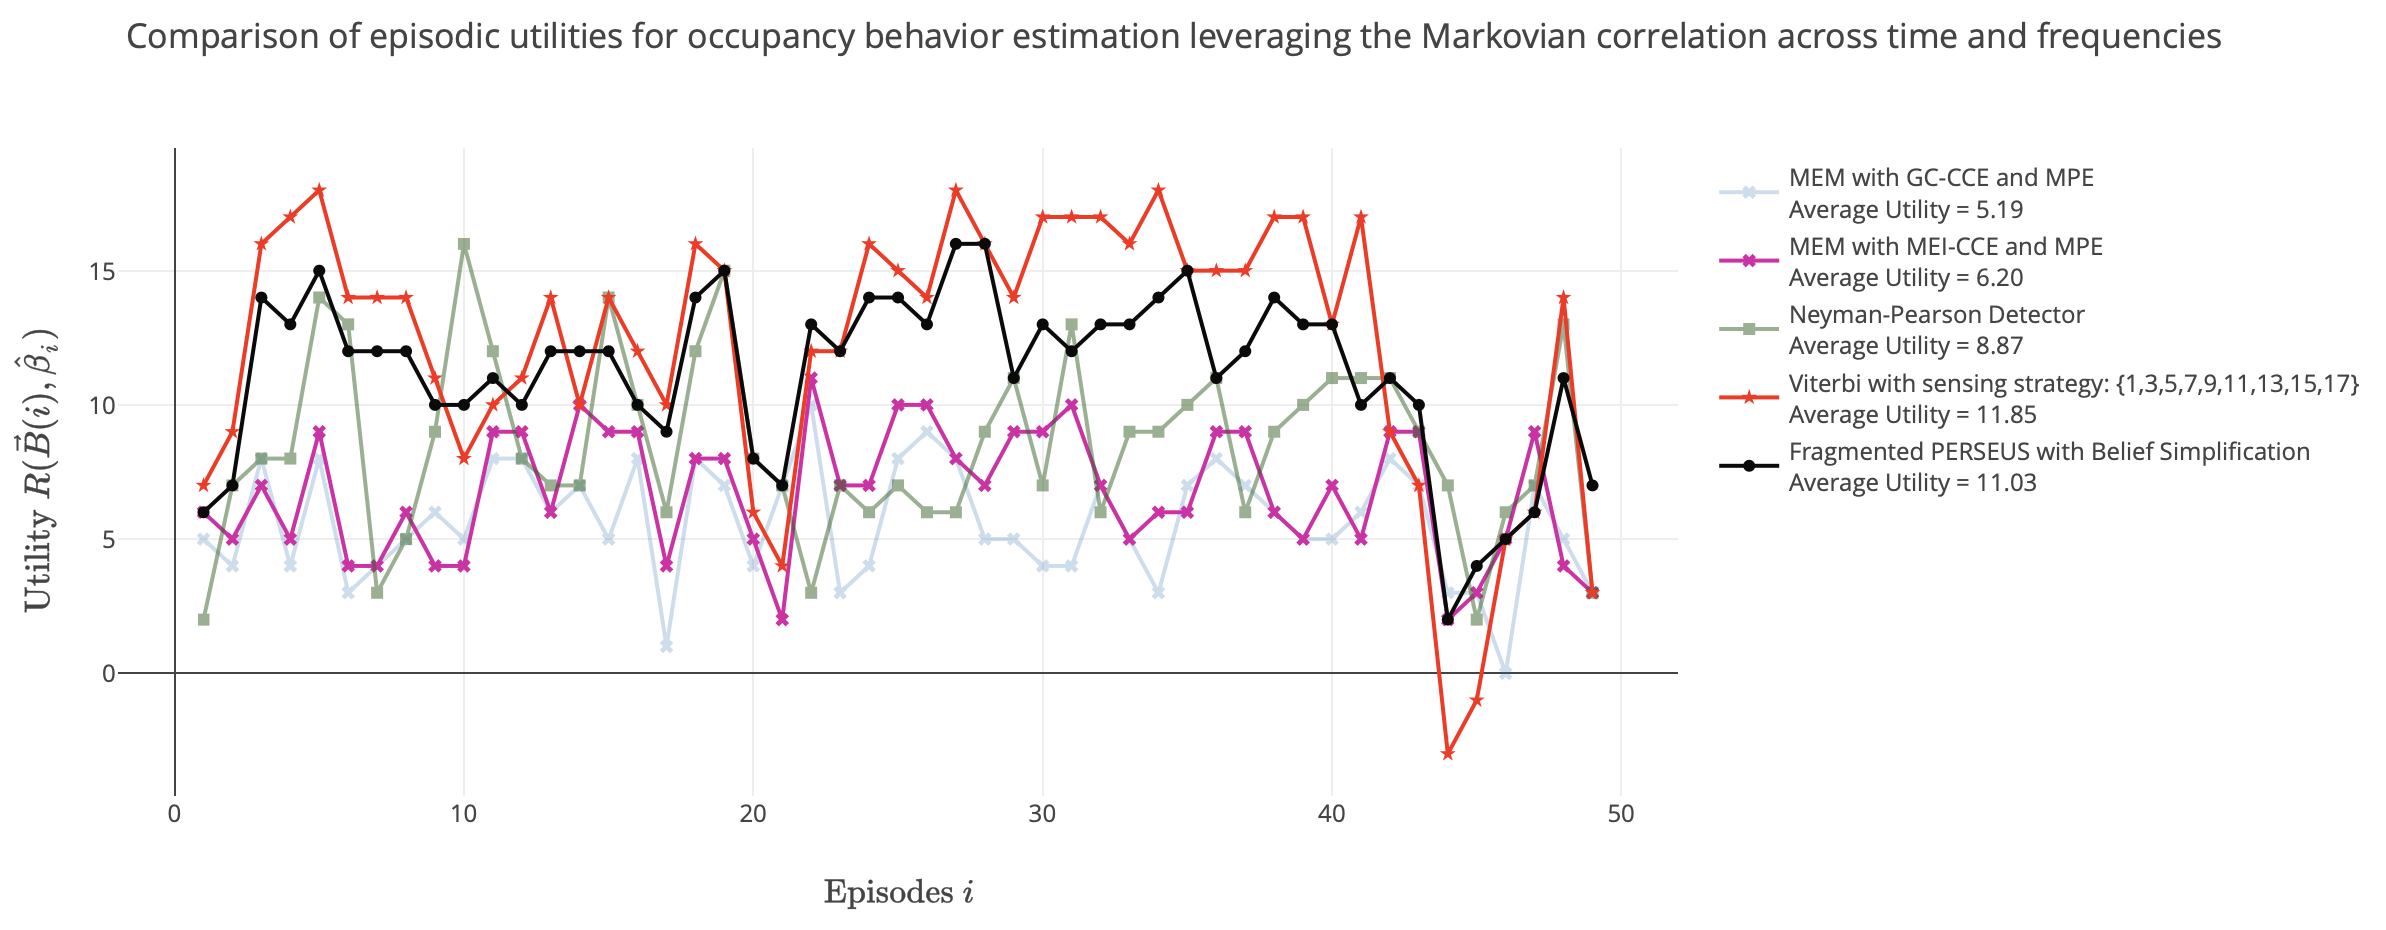
\includegraphics[width=.8\linewidth]{ComparisonWithSoA.png}
    \caption{The evaluation of the proposed framework against a medley of approaches in the state-of-the-art}
    \label{fig:7}
\end{figure}
In this paper, we formulate the optimal spectrum sensing and access problem in an AWGN observation model with multiple licensed users and a cognitive radio node restricted in terms of its sensing capabilities, as a POMDP. In a radio environment wherein the occupancy behavior of the incumbents is correlated across time and frequencies, we present a consolidated framework that employs the Expectation-Maximization algorithm to estimate the transition model of this occupancy behavior and leverage a fragmented PERSEUS algorithm with belief update heuristics to simultaneously solve for the optimal spectrum sensing and access policy. Through system simulations, we illustrate in Fig. \ref{fig:7} that our framework, in terms of the average utility obtained per time-step $i$, outperforms the existing correlation-coefficient based state-of-the-art by 78\%; surpasses Neyman-Pearson based occupancy detection schemes that fail to exploit the correlation across time and frequencies by 24\%; and matches the performance attained by standard MAP-estimators which possess the transition model statistics as an apriori.
\bibliographystyle{IEEEtran}
\bibliography{ref}
\end{document}